\documentclass[a4paper,14pt]{article}

\usepackage[utf8]{inputenc}
\usepackage[russian]{babel}
\usepackage{graphicx}
\usepackage{caption}
\usepackage{float}
\usepackage{subcaption}
\usepackage{array}
\usepackage[left=2cm,right=2cm,top=2cm,bottom=3cm]{geometry}
\usepackage{multicol}
\usepackage[russian]{babel}
\usepackage{tikz}
\usepackage{caption}

\usepackage{blindtext}
\usepackage{graphicx}
\usepackage{amsmath}


\begin{document}
    
    % 3 pictures
    \begin{figure}[H]
        
        \begin{subfigure}[b]{0.3\textwidth}
            \centering
            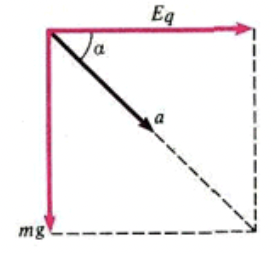
\includegraphics[width=\textwidth]{pic9.png}
            \captionsetup{labelformat=empty,justification=raggedright,singlelinecheck=false}
            \caption{\textbf{\textit{Рис. 9}}}
        \end{subfigure}
        \hfill
        \begin{subfigure}[b]{0.3\textwidth}
            \centering
            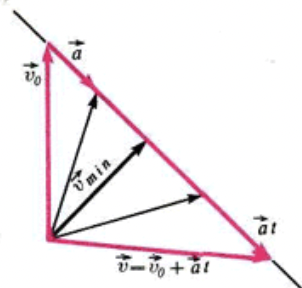
\includegraphics[width=\textwidth]{pic10.png}
            \captionsetup{labelformat=empty,justification=raggedright,singlelinecheck=false}
            \caption{\textbf{\textit{Рис.10}}}
        \end{subfigure}
        \hfill
        \begin{subfigure}[b]{0.35\textwidth}
            \centering
            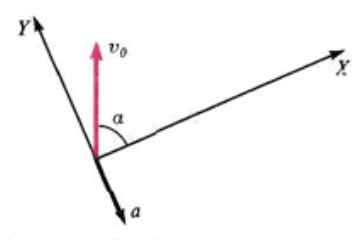
\includegraphics[width=\textwidth]{pic11.png}
            \captionsetup{labelformat=empty,justification=raggedright,singlelinecheck=false}
            \caption{\textbf{\textit{Рис.11}}}
        \end{subfigure}
    \end{figure}
    
    % text start
    \begin{multicols}{2}
        
        \noindent\textbf{Чтобы найти скорость шарика перед вторым ударом (т.е. через время $\tau$) запишем в проекциях на наши оси уравнение (1):}
        
        \begin{center}
            \noindent $U_x = U_{0_x} + g_xt$,
        
            \noindent $U_y = U_{0_y} + g_yt$.
        \end{center}
        
        \noindent\textbf{Подставляя} $t=\tau=2U_y/(-g_y)$\textbf{, получим, что перед вторым ударом} $U_y=-U_{0_y}$ \textbf{и, следовательно, сразу после удара} $U_y=U_{0_y}$\textbf{. Этот результат позволяет облегченно вдохнуть - дальше можно не считать. Так как время между ударами зависит только от $U_{0_y}$, все удары происходят через одинаковое время.}
        
        \textbf{Ответить на вопрос задачи теперь удобнее всего, нарисовав друг под другом графики зависимостей координат шарика от времени (рис. 8). Шарик вернется в ту же точку, если в некоторый момент $x=y=0$, что  может быть только если $T=n\tau$, где n - целое число. Итак,}
        
        \begin{center}
            $\frac{2U_0\cos\beta}{g\sin{\alpha}} = n\frac{2U_0\sin\beta}{g\cos{\alpha}}$,     
        \end{center}
        
        \noindent\textbf{откуда}
        
        \begin{center}
            $\ctg{\beta} = n \tg{\alpha}$.
        \end{center}
        
        \textbf{Интересно, что при четных и при нечетных n шарик ведет себя несколько по-разному. При четных n средний удар шарика (всего ударов $n + 1$) происходит перпендикулярно плоскости, и шарик возвращается обратно по той же траектории. Если же n нечетно, то после половины ударов шарик летит вертикально вверх, падает обратно, и также возвращается, повторяя весь пройденный путь.}
        
        \textbf{З а д а ч а\quad3. \textit{В область пространства, где создано горизонтальное электрическое}}
        
        \columnbreak
        
        \noindent\textbf{\textit{поле с напряженностью $\vec{E}$, запускают шарик, масса которого m, а заряд q, со скоростью $\vec{U_0}$, направлвенной вертикально вверх. Какова минимальная скорость шарика в процессе движения?}}
        
        \textbf{Вас не удивило присутствие здесь <<электрической>> задачи? Нет? И правильно, эта задача, конечно же, имеет прямое отношение к кинематике.}
        
        \textbf{Обсудим два решения.}
        
        \textbf{Р е ш е н и е\quad1. На шарик в полете действуют две силы: сила тяжести $m\vec{g}$ и электрическая сила $\vec{E}q$ (рис. 9). По второму закону Ньютона ускорение шарика постоянно и равно}
        
        \begin{center}
            $\vec{a} = \frac{\vec{E}q + m\vec{g}}{m}$. 
        \end{center}
        
        \noindent\textbf{При этом}
        
        \begin{center}
            $a = |\vec{a}| = \frac{\sqrt{(Eq)^2 + (mg)^2}}{m}$. 
        \end{center}
        
        \noindent\textbf{На рисунке 10 показано, как изменяется со временем вектор скорости шарика (<<нарисована>> формула (1)). Ясно, что минимальная скорость будет через время}
        
        \begin{center}
            $t = \frac{U_0\sin{\alpha}}{\alpha}$,
        \end{center}
        
        \noindent\textbf{и ее величина будет равна}
        
        \begin{center}
            $U_{min} = U_0 \cos{\alpha} = U_0 \frac{Eq}{\sqrt{(Eq)^2 + (mg)^2}}$.
        \end{center}
        
        \textbf{Если вам хочется побольше формул, можно сделать по-другому.}
        
        \textbf{Р е ш е н и е\quad2. Направим оси координат перпендикулярно и параллельно ускорению (рис. 11) и запишем уравнение (1) в проекциях на эти оси:}
        
    \end{multicols}
    
\end{document}